
\begin{frame}
  \frametitle{Flattened \kd trees}
  \framesubtitle{Introduction}

  \begin{itemize}
    \item Similar to traditional \kd trees, partition space using hyperplanes that are 
      fixed w.r.t. one dimension of the original space
    \item Take a parameter $b$, the branching factor which must be a power of two, and
      organize $b-1$ hyperplanes into a single node in a BST
    \item Each node has up to $b$ children, each of which accounts for a disjoint subspace 
      of the parent's space
  \end{itemize}

\end{frame}

\begin{frame}
  \frametitle{Flattened \kd trees}
  \framesubtitle{Example: $k=3$ and $b=8$}
  
  \begin{figure}
    \centering
    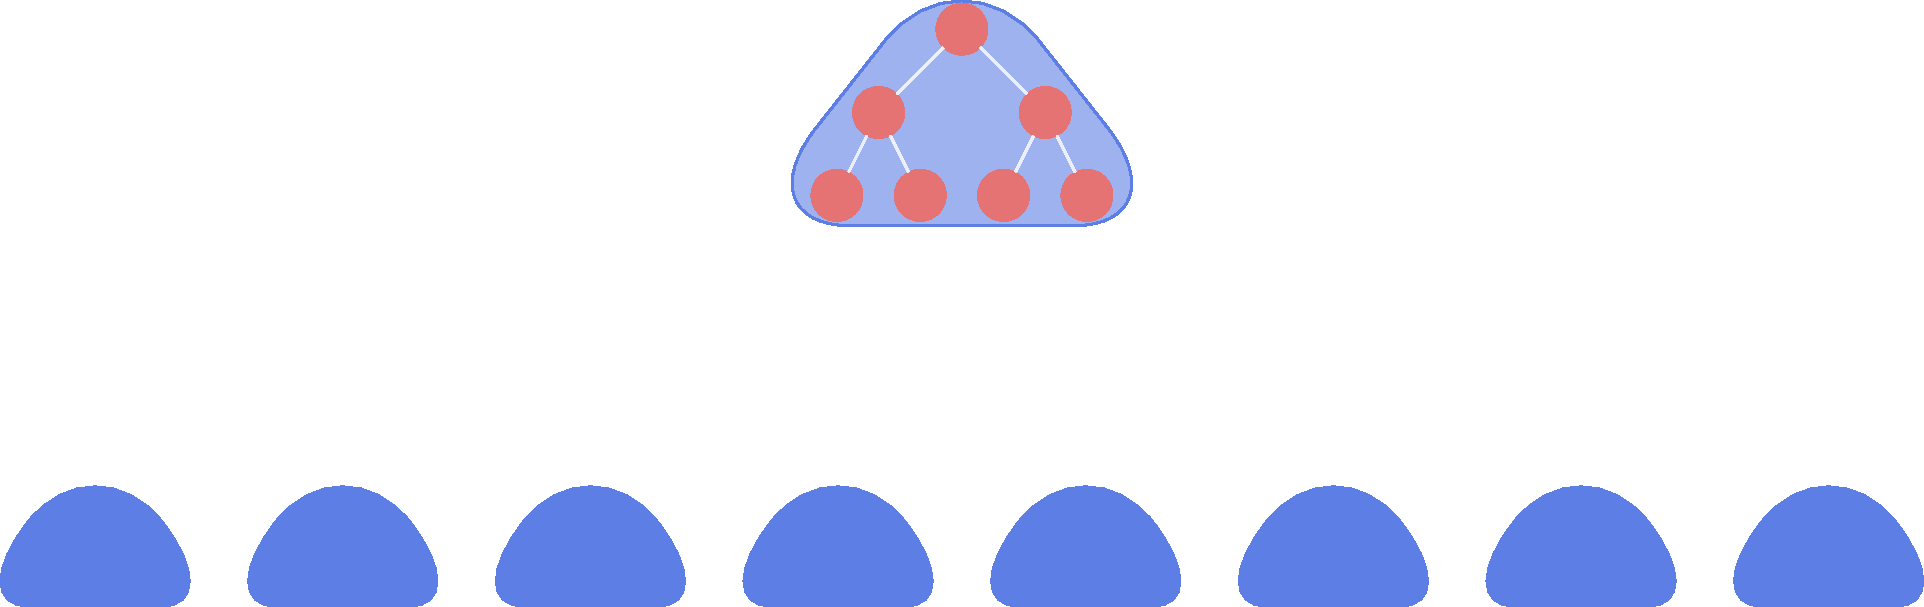
\includegraphics[width=\textwidth]{flatkdtree.pdf}
  \end{figure}

\end{frame}

\begin{frame}
  \frametitle{Flattened \kd trees}
  \framesubtitle{Advantages}

  \begin{itemize}
    \item Increased dimensionality reduces height of tree
    \item Packed hyperplanes allow for more powerful look ahead to adjacent
      spaces during search
  \end{itemize}

\end{frame}

\begin{frame}
  \frametitle{Flattened \kd trees}
  \framesubtitle{Disadvantages}

  \begin{itemize}
    \item Additional computation required at each node during search
    \item More complex conditions during nearest neighbor adjacent subspace
      checks require additional information to be saved per node
  \end{itemize}

\end{frame}

\begin{frame}
  \frametitle{Flattened \kd trees}
  \framesubtitle{NN adjaceny check}

  \begin{figure}
    \centering
    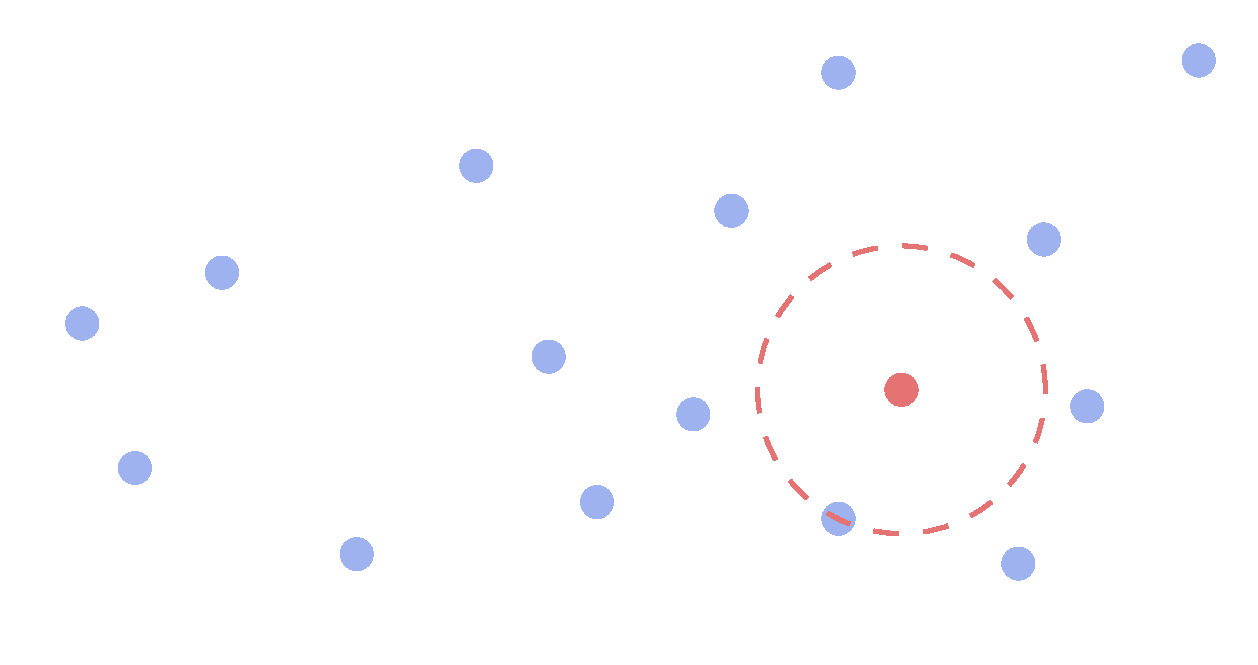
\includegraphics[width=0.85\textwidth]{nn_adjaceny_complex.pdf}
  \end{figure}

\end{frame}

\begin{frame}
  \frametitle{Flattened \kd trees}
  \framesubtitle{Initial results}

  \color{white}
  (On test of 1000 searches)
  Graph showing run time of different branch factors
  Graph showing number of pointer dereferences

\end{frame}

\begin{frame}
  \frametitle{Flattened \kd trees}
  \framesubtitle{Initial results}

  \color{white}
  (On test of 1000 searches)
  Graph showing L1 Data Cache misses

\end{frame}

\begin{frame}
  \frametitle{Flattened \kd trees}
  \framesubtitle{Shortcomings}

  \begin{itemize}
    \item Despite reduced pointer dereferences, still visiting significant amount of nodes
    \item Naive implementation incurs significant computational costs 
       Maybe add in list of thinkgs that were contributing to this
  \end{itemize}

\end{frame}
